\documentclass{beamer}

\usetheme[]{Rochester}
\usecolortheme{beaver}
\usepackage[latin1]{inputenc}
\usepackage{graphics}

\author{Will Webberley}
\date{Autumn 2014}
\institute[COMSC]{Cardiff School of Computer Science and Informatics}



\title{Heuristic Evaluation}
\subtitle{CM2101: Human-Computer Interaction}

\begin{document}

\frame{\titlepage}

\frame{
    \frametitle{Heuristic evaluation}
    \begin{itemize}
        \item Another type of evaluation (after user evaluation)
        \item Performed by an \alert{expert} (rather than normal users)
        \item Essentially, the UI is thoroughly inspected and \alert{usability problems are listed}
        \item \textit{Every} problem should be listed
        \item May need to go through twice (allowing a time to get the hang of the system)
        \item The heuristics are used for \alert{justifying} the problems
    \end{itemize}
    \vskip20pt
    Many aspects of interactions are subjective (e.g. ``I don't like the colours.''), but heuristics can help prevent subjective opinion.
}

\frame{
    \frametitle{Heuristic evaluation: uses}
    \begin{columns}
        \column{.5\textwidth}
            \begin{itemize}
                \item Usable in the `evaluation' phase of the iterative interaction development cycle
                \item Useful on low- and high-fidelity prototypes
                \begin{itemize}
                    \item Sketches and paper prototypes
                    \item Buggy and more complete implementations
                \end{itemize}
                \item However, probably harder with low-fi prototypes
                \begin{itemize}
                    \item Some more interactive functionality cannot be evaluated
                \end{itemize}
            \end{itemize}
        \column{.5\textwidth}
            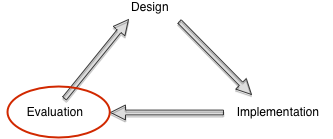
\includegraphics[width=6cm]{media/cycle_2.png}   
    \end{columns}
}

\frame{
    \frametitle{Heuristic evaluation: formal process}
    \textbf{4 main stages}
    \begin{enumerate}
        \item Training
        \begin{itemize}
            \item Design team meet evaluator(s)
            \item Design team introduce application
            \item Design team explain domain, audience, scenarios of use
        \end{itemize}
        \item Evaluation
        \begin{itemize}
            \item Evaluators (if multiple) work separately
            \item A written report is generated
            \item Ovserver can record oral comments
            \item Focus is on simply listing usability problems
        \end{itemize}
        \item Severity rating
        \begin{itemize}
            \item Evaluators work together
            \item Severity rating applied to each problem
            \item Problems prioritised by severity
        \end{itemize}
        \item Debrief
        \begin{itemize}
            \item Evaluators meet back with design team
            \item Problems and solutions discussed
        \end{itemize}
    \end{enumerate} 
}

\frame{
    \frametitle{Heuristic evaluation: evaluation stage}
    \textbf{Stage 2 from `formal process' slide}
    \begin{block}{Evaluation process}
        \begin{enumerate}
            \item Identify a system to be evaluated
            \item Identify a set of heuristics
            \item Go through the interface once to get a feel of its layout and the options and tasks available
            \item Go through the interface again more thoroughly
            \item List all usability problems identified
            \item Explain, assess, and justify each problem using the heuristics
        \end{enumerate}
    \end{block}   
}

\frame{
    \frametitle{Heuristic evaluation: hints}
    \begin{itemize}
        \item Use multiple evaluators
        \begin{itemize}
            \item Different evaluators find different problems
            \item More evaluators: more problems identified (though this is logarithmic)
            \item Neilsen recommends 3-5 evaluators (a bit like `think aloud')
        \end{itemize}
        \item Use heuristic evaluation with user evaluation
        \begin{itemize}
            \item Each method identifies different issues
            \item Heuristic evaluation can be cheaper (no room setup, no separate facilitator, etc.)
        \end{itemize}
        \item Use an observer, if necessary
        \begin{itemize}
            \item Observer can provide help if evaluator gets stuck
            \item This is \textit{not} allowed in user evaluations
        \end{itemize}
    \end{itemize}
}

\frame{
    \frametitle{Heuristic evaluation: guidelines}
    \begin{itemize}
        \item Generated report cards (see later) need to communicate to \alert{different types of people}
        \begin{itemize}
            \item Design team
            \item Developers
            \item Managers
        \end{itemize}
        \item Include some \alert{positive comments} as wll as problems (especially if they can be used as comparisons)
        \begin{itemize}
            \item Navigation bar has logo in same place in each activity (addresses \textit{Consistency and Standards} heuristic)
        \end{itemize}
        \item Recommendations should be \alert{clear}
        \begin{itemize}
            \item Bad: `buttons have non-obvious functions'
            \item Good: `icon-only buttons should use more appropriate icons on screen $x$'
        \end{itemize}
        \item Recommendations should be \alert{specific}
        \begin{itemize}
            \item Bad: `the text on screen $y$ is not readable'
            \item Good: `the text on screen $y$ should be in 13pt Helvetica Neue as on screen $z$'
        \end{itemize}
    \end{itemize}
}

\frame{
    \frametitle{Heuristic vs. user evaluation}
    Example of user evaluation: `think aloud' (see last week's slides)
    \begin{itemize}
        \item In both cases, evaluators are not typical users
        \item Though, in user evaluations then this is likely to be closer
        \item User evaluation can often be opinion-driven
        \item User evaluation depends on the evaluator's experience with systems in general
        \item Heuristic evaluation often identifies problems missed by user evaluation
        \begin{itemize}
            \item Inconsistent colours and fonts
            \item Lack of feedback and visibility
            \item Layout of interface
        \end{itemize}
        \item User evaluation represents the gold standard for usability
    \end{itemize}
}

\frame{
    \frametitle{Revisiting Neilsen's heuristics}
    \begin{enumerate}
        \item Visibility of system status
        \begin{itemize}
            \item System should inform users about what's going on internally.
        \end{itemize}
        \item Match between system and real world
        \begin{itemize}
            \item System should speak the user's language and allow functions in a logical order.
        \end{itemize}
        \item User control and freedom
        \begin{itemize}
            \item Provide an `emergency exit' (e.g. by allowing an `undo' action)
        \end{itemize}
        \item Consistency and standards
        \begin{itemize}
            \item Ensure that different words or actions don't mean the same thing. Follow the platform guidelines.
        \end{itemize}
        \item Error prevention
        \begin{itemize}
            \item As well as using good error messages, try and prevent errors from happening.
        \end{itemize}
    \end{enumerate}
}

\frame{
    \frametitle{Revisiting Neilsen's heuristics}
    \begin{enumerate}
        \setcounter{enumi}{5}
        \item Recognition rather than recall
        \begin{itemize}
            \item Reduce users' memory loads by making actions and options visible. Use standard practices.
        \end{itemize}
        \item Flexibility and efficiency
        \begin{itemize}
            \item Cater to both expert and unexperienced users by making it faster to use for experts.
        \end{itemize}
        \item Aesthetic and minimalist design
        \begin{itemize}
            \item Do not display irrelevant information. Keep interface concise and provide contextually relevant actions.
        \end{itemize}
        \item Help users recognise, diagnose, and recover from errors
        \begin{itemize}
            \item Use English, avoid error codes, constructively provide a solution.
        \end{itemize}
        \item Help and documentation
        \begin{itemize}
            \item If you \textit{do} need documentation, make it easily searchable and task-focussed.
        \end{itemize}
    \end{enumerate}
}



\frame{
    \frametitle{Heuristic evaluation: small example}
    \centering
    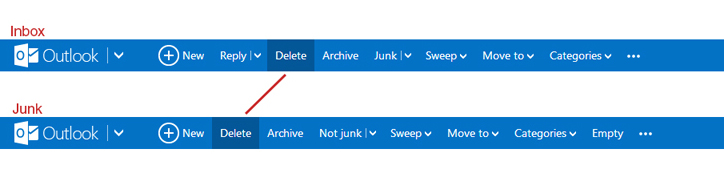
\includegraphics[width=11cm]{media/outlook.jpg}    
    \vskip20pt
    Same actions in different places in very similar views. This violates \alert{consistency} and \alert{recognition \& recall}.
}

\frame{
    \frametitle{Introducing severity ratings}
    \textbf{Contributing factors}
    \begin{itemize}
        \item How common is the problem?
        \begin{enumerate}
            \item Once
            \item Rarely
            \item Frequently
        \end{enumerate}
        \item How impactful is the problem?
        \begin{enumerate}
            \item Small impact
            \item Medium impact
            \item Large impact
        \end{enumerate}
        \item How persistent is the problem?
        \begin{enumerate}
            \item Easy to fix
            \item Long fix
        \end{enumerate}
    \end{itemize}
}

\frame{
    \frametitle{Severity ratings: scale}
    \textbf{Applying a rating scale} 
    \begin{enumerate}
        \item \alert{Cosmetic}: fix not necessary
        \item \alert{Minor}: fix required at low priority
        \item \alert{Major}: fix required at high priority
        \item \alert{Catasrophic}: fix required within next iteration
    \end{enumerate}
}

\frame{
    \frametitle{Generating reports}
    \textbf{During Stage 2 from `formal process' slide}
    \vskip20pt

    Produce a list of cards, each representing a problem and including:
    \begin{itemize}
        \item The \alert{usability} problem identified
        \item The \alert{heuristic} being violated 
        \item \alert{Description} of the problem and how it violates the heuristic
        \item \alert{Severity}
        \item \alert{Recommendation} (if any at this stage)
        \item Any \alert{additional material}, if necessary
        \begin{itemize}
            \item e.g. screenshots
        \end{itemize}
    \end{itemize}
}

\frame{
    \frametitle{Evaluation card}
    \centering
    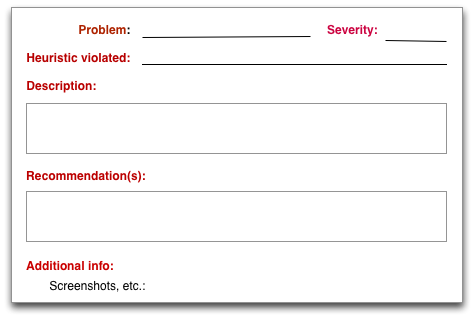
\includegraphics[width=\textwidth]{media/card.png}    
}

\frame{
    \frametitle{Example evaluation interface}
    \centering
    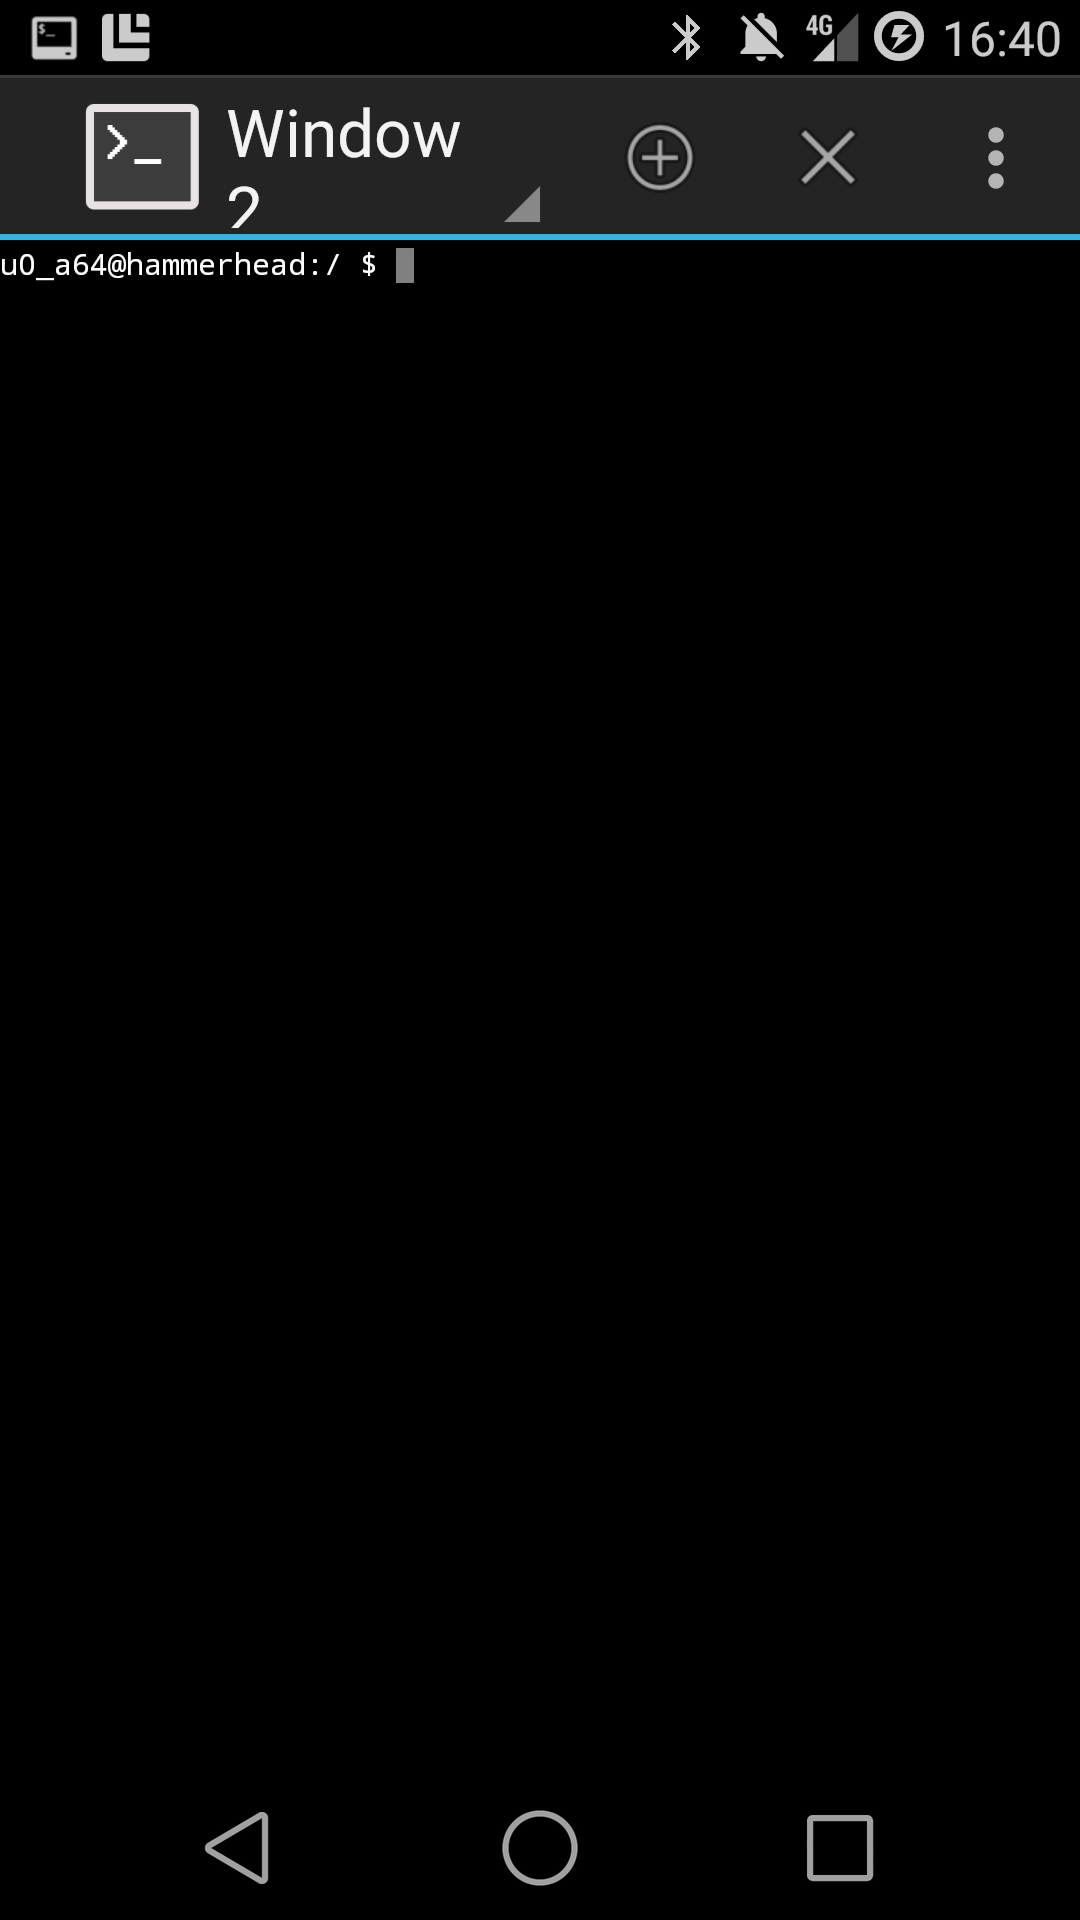
\includegraphics[height=7cm]{media/terminal.png}
}

\frame{
    \frametitle{Example evaluation card}
    \centering
    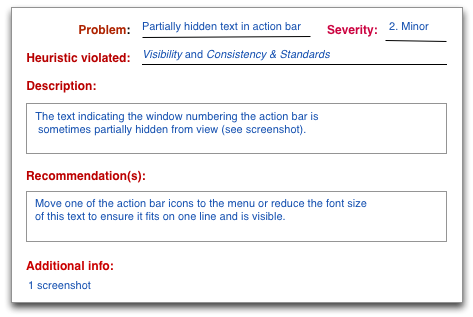
\includegraphics[width=\textwidth]{media/card_2.png}
}

\frame{
    \frametitle{Revision questions}
    \begin{enumerate}
        \item What kind of person performs a heuristic evaluation?
        \item What are the main benefits of heuristic evaluations?
        \item At what stage and how far through interaction development is heuristic evaluation useful?
        \item What are heuristics used for during a heuristic evaluation?
        \item Why is it important that heuristic and user evaluations are \textit{both} used?
        \item Describe the overall process of a heuristic evaluation.
        \item Name and describe 5 of Neilsen's heuristics for usability evaluation. Why are they important?
        \item What should be considered when deciding on the severity of a usability problem?
        \item When generating report cards, what information is important to capture?
    \end{enumerate}
}

\frame{
    \frametitle{Summary}
    \begin{itemize}
        \item The importance and uses of heuristic evaluation
        \item The overall evaluation method
        \item The heuristic evaluation process
        \item Comparison between heuristic and user evaluation techniques
        \item Neilsen's heuristics
        \item Usability problem severities
        \item Generating heuristic evaluation reports
    \end{itemize}
}
    
\end{document}
